\section{Results}
\label{sec:results}

To validate the proposed exploration strategy, we implemented the formulations
and algorithms discussed in Sections~\ref{sec:information_theoretic_objective}-\ref{sec:state_estimation}
in a high-fidelity C++ simulation environment. The simulator assumes a ground robot
constrained to a 2D horizontal plane, which is equipped with a noisy laser scanner (range $
= 30$ m, $\sigma = 0.1$ cm), and IMU. The robot's motion is governed by a 13-state nonlinear model of skid-steer dynamics controlled by velocity and yaw rate commands. The velocity command is computed using a proportional-derivative (PD) feedback law on the position error between the robot's current position and current reference point. The yaw rate command is computed based on proportional feedback on the error between the robot's current heading angle and the angle to the reference point. Our simulator generates horizontal laser scans
from a meshed point cloud input, and generates IMU observations according to the true
state of the robot. Prior to evaluating CSQMI or building an RRT, we populate a map using recent laser scans
and localize with respect to it using a custom SLAM implementation that was
developed prior to this project. Our SLAM implementation leverages ICP for laser
odometry~\cite{pomerleau2013comparing}, a histogram filter for
localization~\cite{thrun2005probabilistic}, and a custom 3D mapping framework.


To evaluate performance of the proposed exploration framework, we consider two simulation environments, shown in Fig.~\ref{fig:maps}. Figure~\ref{fig:smallmap_snapshots} shows a series of snapshots of the robot navigating the smaller map. The robot is initially unaware of the map layout and must construct it while driving. The occupancy grid is updated at 10 Hz, and the planner replans online at 1 Hz to use the updated map information. This enables it to successfully plan around obstacles as they are detected. Moreover, the tree of candidate trajectories that are considered at each planning iteration accurately identifies regions of the map that have not yet been explored and therefore would result in large information gains (indicated by the green nodes in the tree). Regions of the map that have already been observed will yield significantly less information, and this approach accurately captures this effect (indicated by the red nodes in the tree). We observe similar performance on the larger environment, as illustrated in Fig.~\ref{fig:largemap_snapshots}. Due to the speed of the RRT-based approach, the planner is able to consider candidate paths extending into a large portion of the environment at each step, allowing it to automatically identify and explore the most salient regions even in an expansive and more complex environment.

\begin{figure}[t]
	\centering
	\begin{subfigure}{0.49\textwidth}
	\centering
	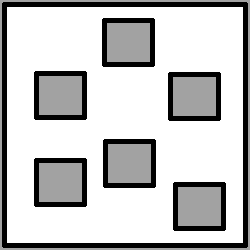
\includegraphics[height=1.35in]{square.png}
	\caption{Small test environment\label{fig:square_map}}
	\end{subfigure}
		
	\vspace*{0.1in}
		
	\begin{subfigure}{0.49\textwidth}
	\centering
	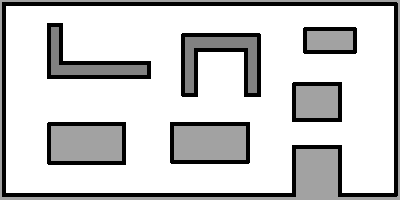
\includegraphics[height=1.35in]{rectangle_medium.png}
	\caption{More complex test environment\label{fig:rectangle_medium_map}}
	\end{subfigure}
	\caption{Layouts of the environments used to test the proposed exploration technique. \label{fig:maps}}
\end{figure}

\begin{figure*}[t]
  \centering
	\begin{subfigure}{0.24\textwidth}
	\centering
	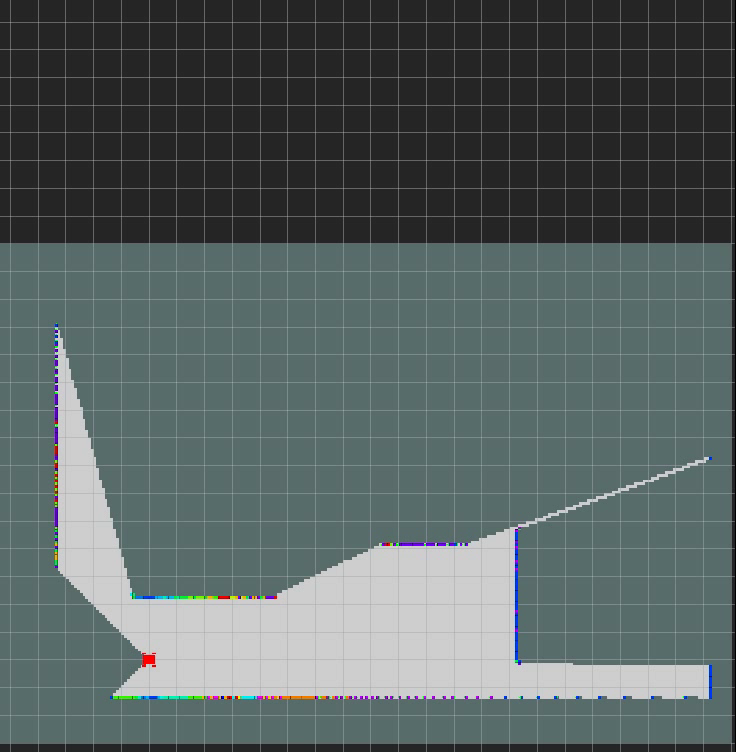
\includegraphics[width=1.0\textwidth]{smallmap_frame1.png}
	\caption{Initially observed map\label{fig:smallmap_frame1}}
	\end{subfigure}
	\begin{subfigure}{0.24\textwidth}
	\centering
	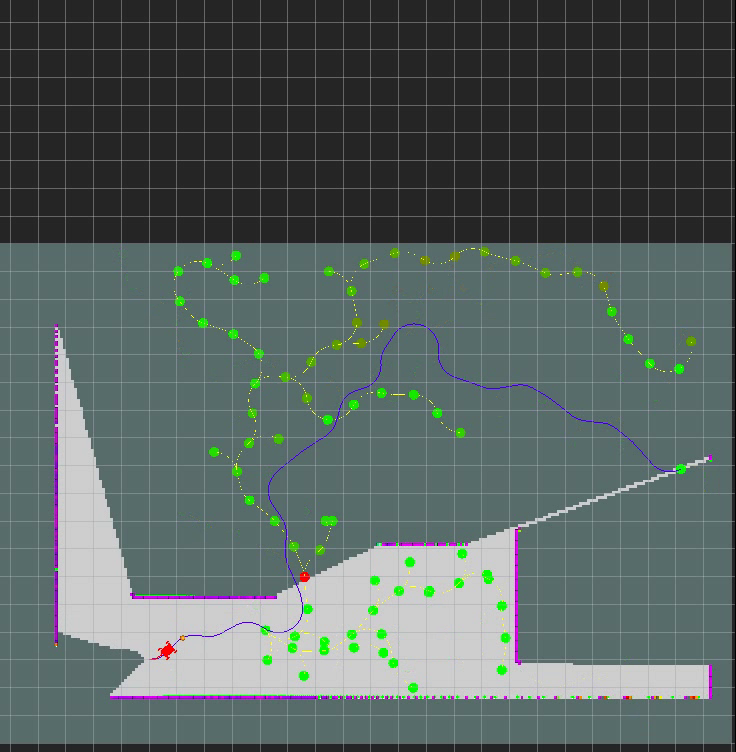
\includegraphics[width=1.0\textwidth]{smallmap_frame2.png}
	\caption{Picks path from planning tree\label{fig:smallmap_frame2}}
	\end{subfigure}
	\begin{subfigure}{0.24\textwidth}
	  \centering
	  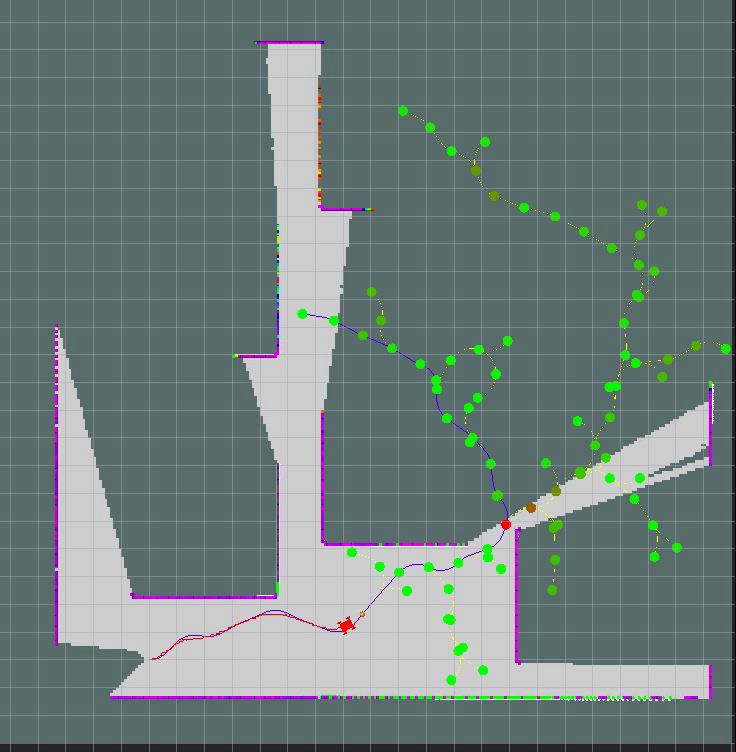
\includegraphics[width=1.0\textwidth]{smallmap_frame3.png}
	  \caption{Plans toward unknown regions\label{fig:smallmap_frame3}}
	\end{subfigure}
	\begin{subfigure}{0.24\textwidth}
	 \centering
	 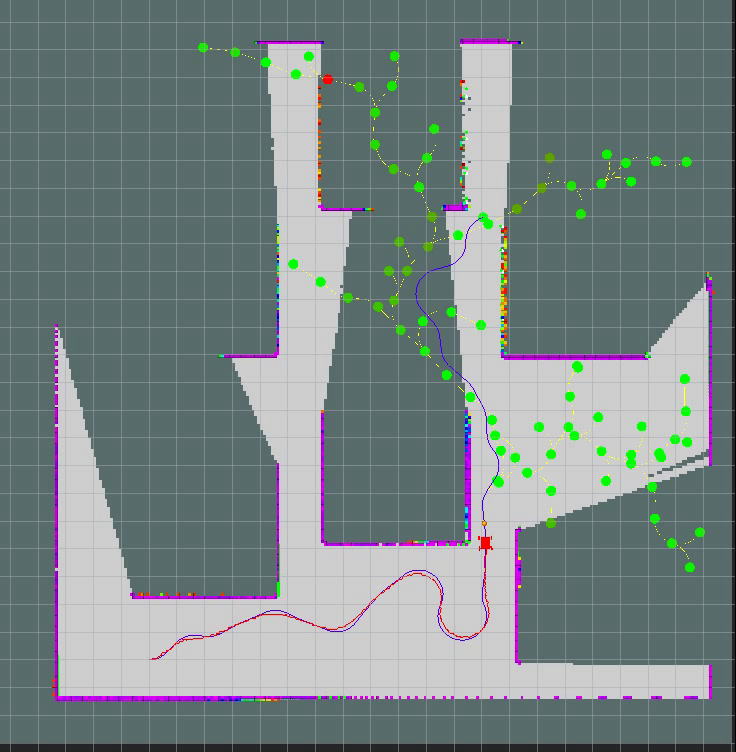
\includegraphics[width=1.0\textwidth]{smallmap_frame4.png}
	 \caption{Map significantly expanded \label{fig:smallmap_frame4}}
	\end{subfigure}
	
	\vspace*{0.1in}

	\begin{subfigure}{0.24\textwidth}
	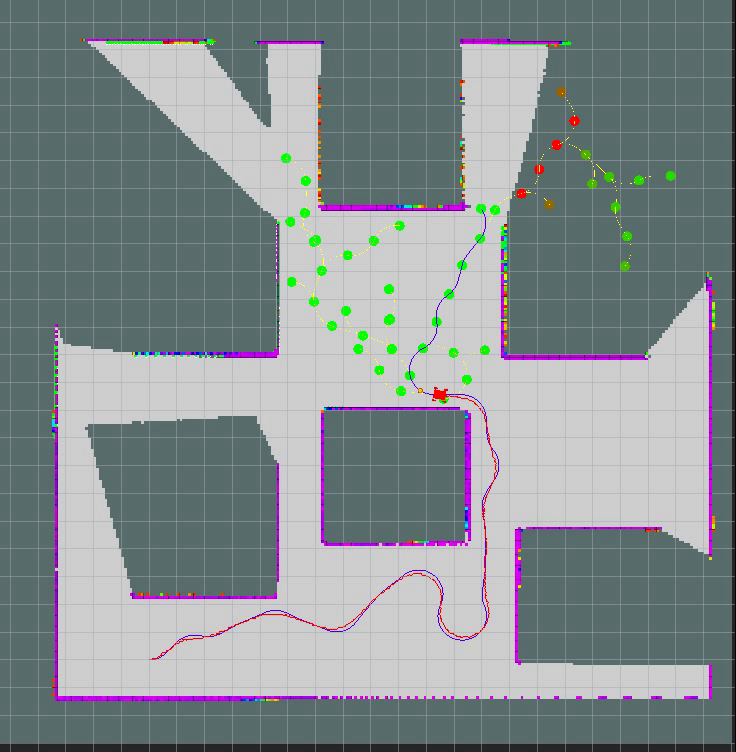
\includegraphics[width=1.0\textwidth]{smallmap_frame5.png}
	\caption{Plans around new obstacles\label{fig:smallmap_frame5}}
	\end{subfigure}
	\begin{subfigure}{0.24\textwidth}
	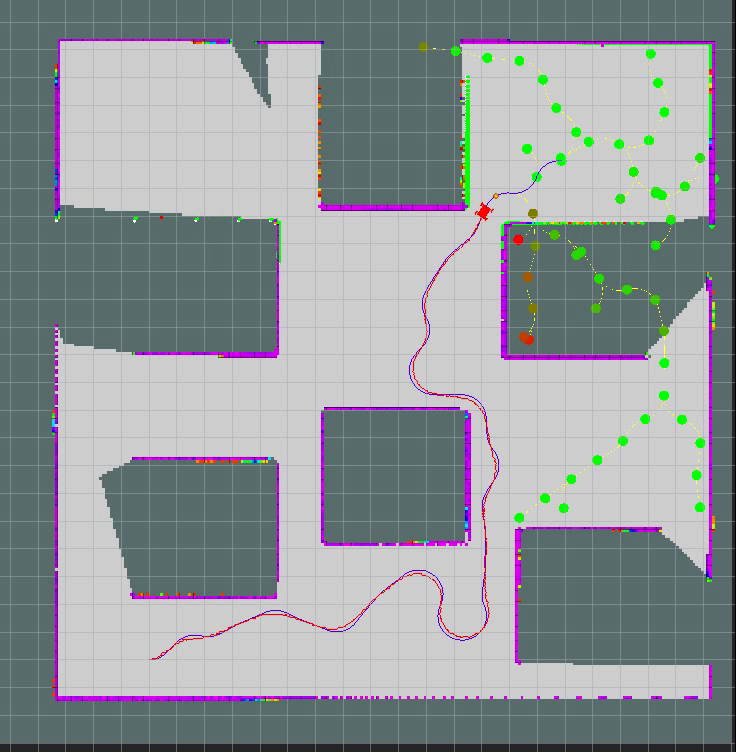
\includegraphics[width=1.0\textwidth]{smallmap_frame6.png}
	\caption{Environment mostly observed\label{fig:smallmap_frame6}}
	\end{subfigure}
	\begin{subfigure}{0.24\textwidth}
	\centering
	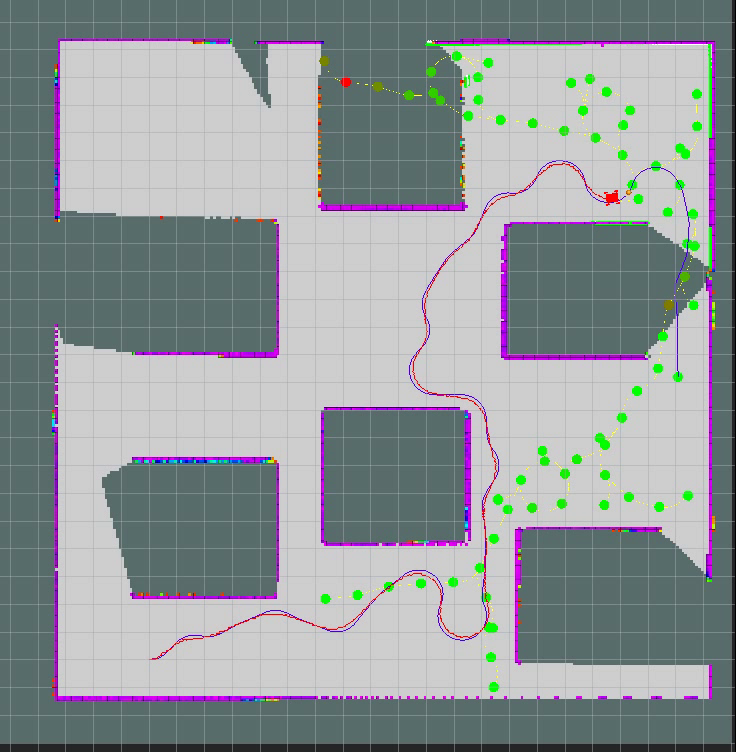
\includegraphics[width=1.0\textwidth]{smallmap_frame7.png}
	\caption{Continues exploring\label{fig:smallmap_frame7}}
	\end{subfigure}
	\begin{subfigure}{0.24\textwidth}
	\centering
	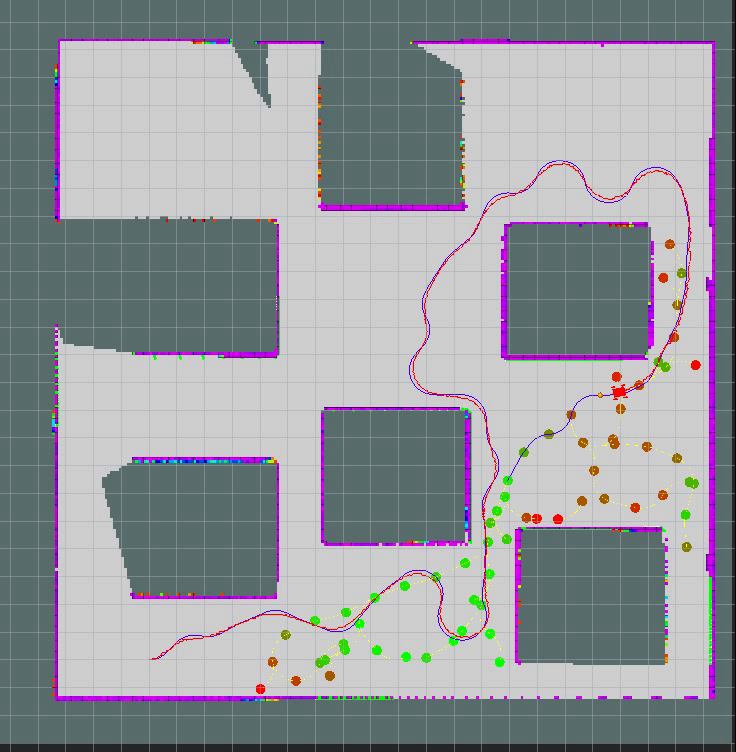
\includegraphics[width=1.0\textwidth]{smallmap_frame8.png}
	\caption{Known areas yield low rewards\label{fig:smallmap_frame8}}
	\end{subfigure}
  \caption{Snapshots of the ground robot exploring an initially unknown environment using information gain to drive planning.  The nodes in the tree are colored according to information gain (green = high, red = low). \label{fig:smallmap_snapshots}}
\end{figure*}


\begin{figure*}[t]
	\centering
	\begin{subfigure}{0.49\textwidth}
	\centering
	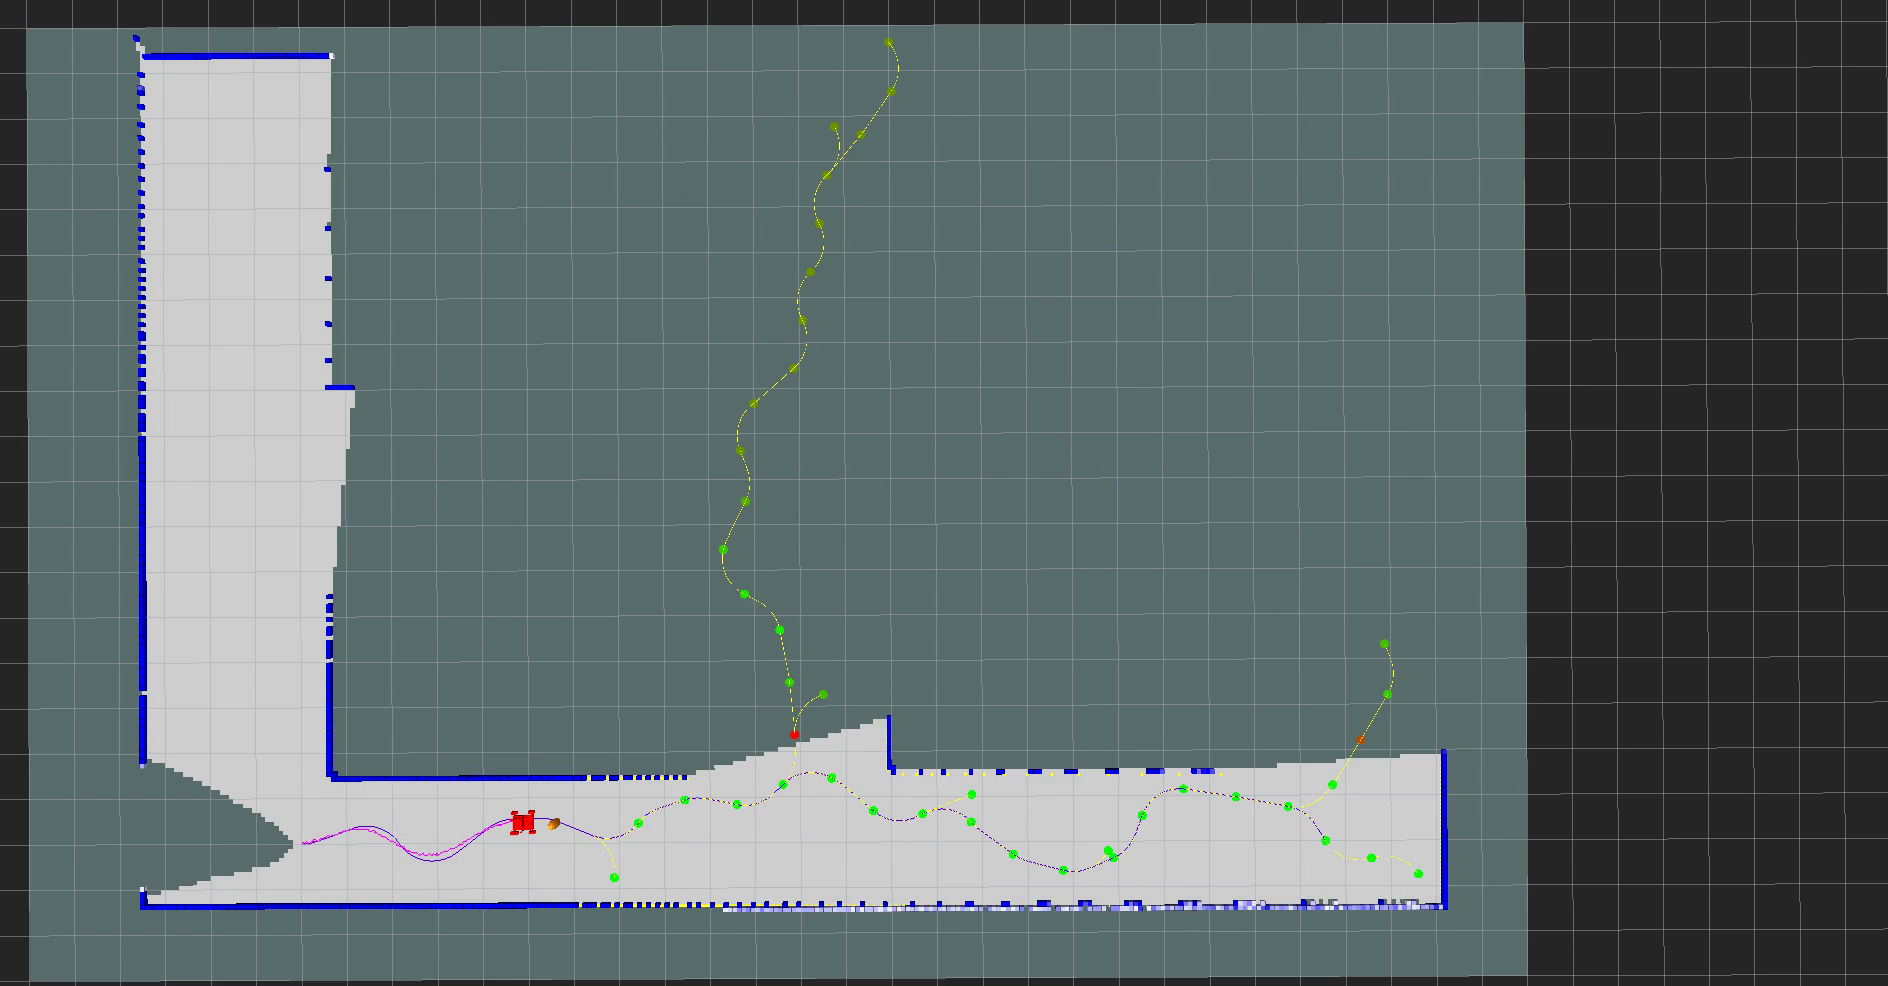
\includegraphics[width=0.9\textwidth]{largemap_frame1.png}
	\caption{Initial exploration guides robot down hallway\label{fig:largemap_frame1}}
	\end{subfigure}
	\begin{subfigure}{0.49\textwidth}
	\centering
	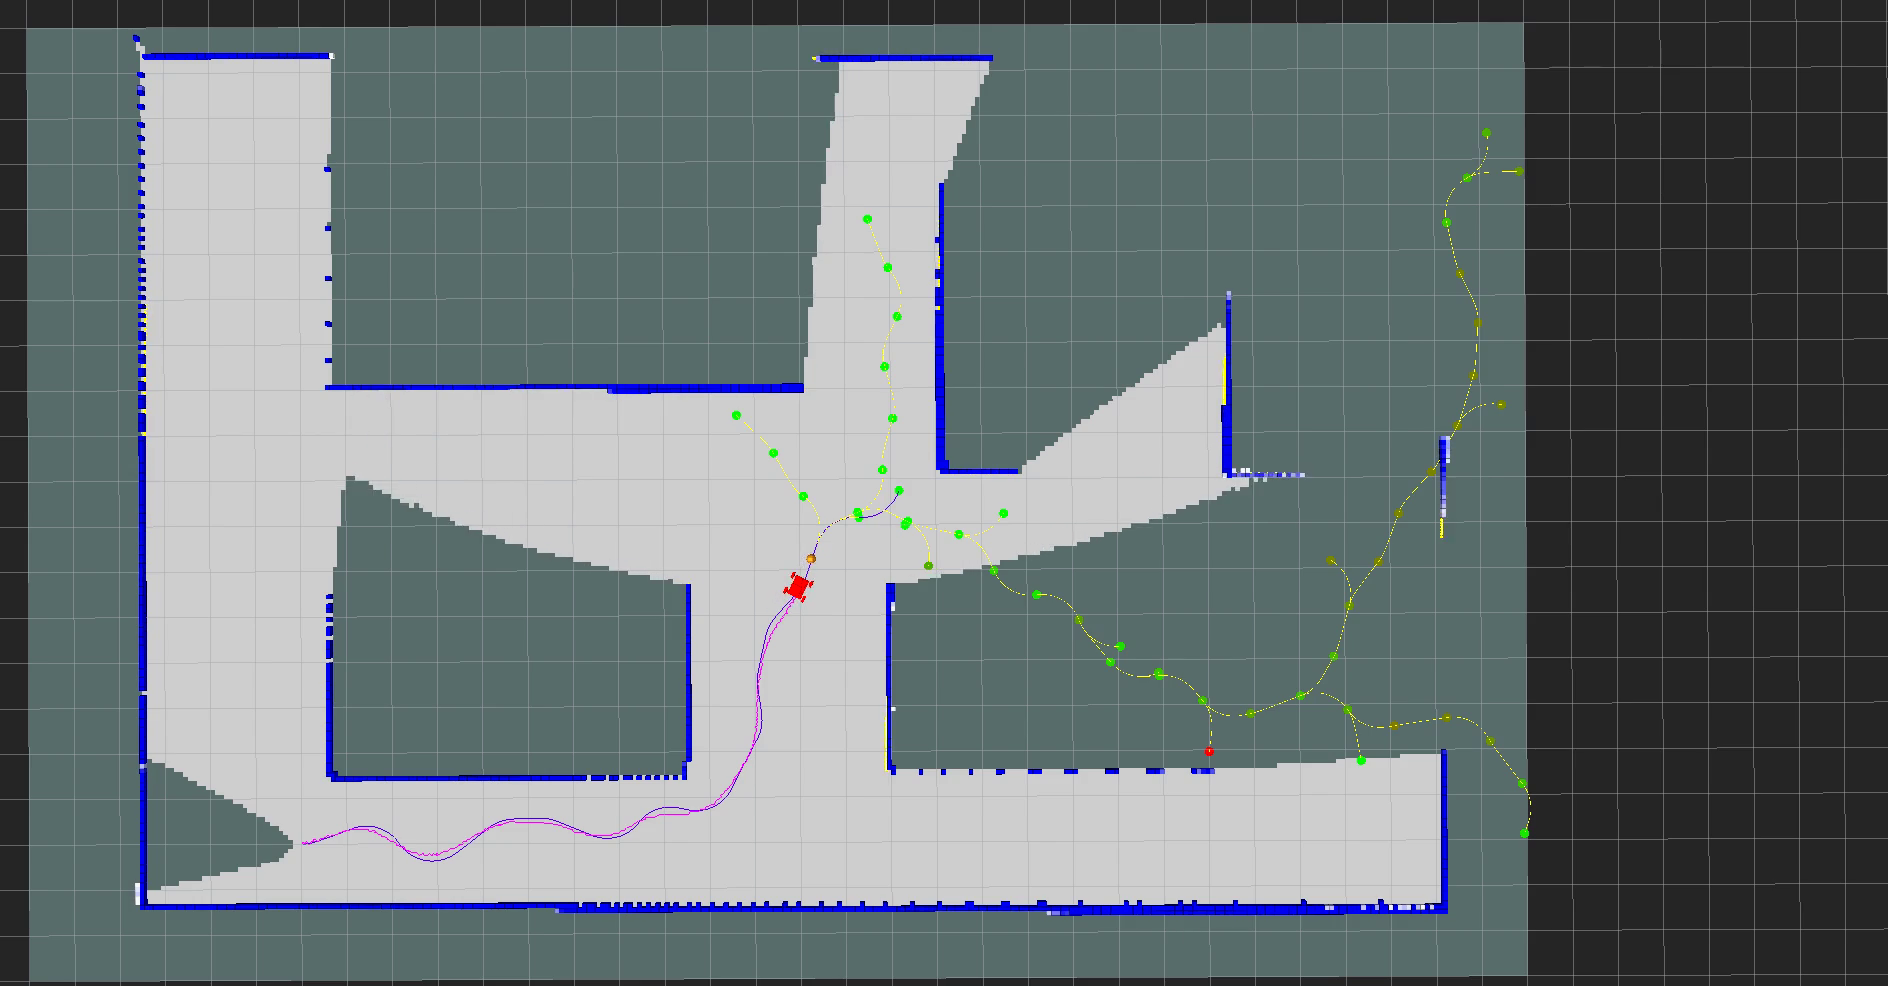
\includegraphics[width=0.9\textwidth]{largemap_frame2.png}
	\caption{High information-gain nodes added near unknown regions\label{fig:largemap_frame2}}
	\end{subfigure}
	
	\vspace*{0.2in}
	
	\begin{subfigure}{0.49\textwidth}
	\centering
	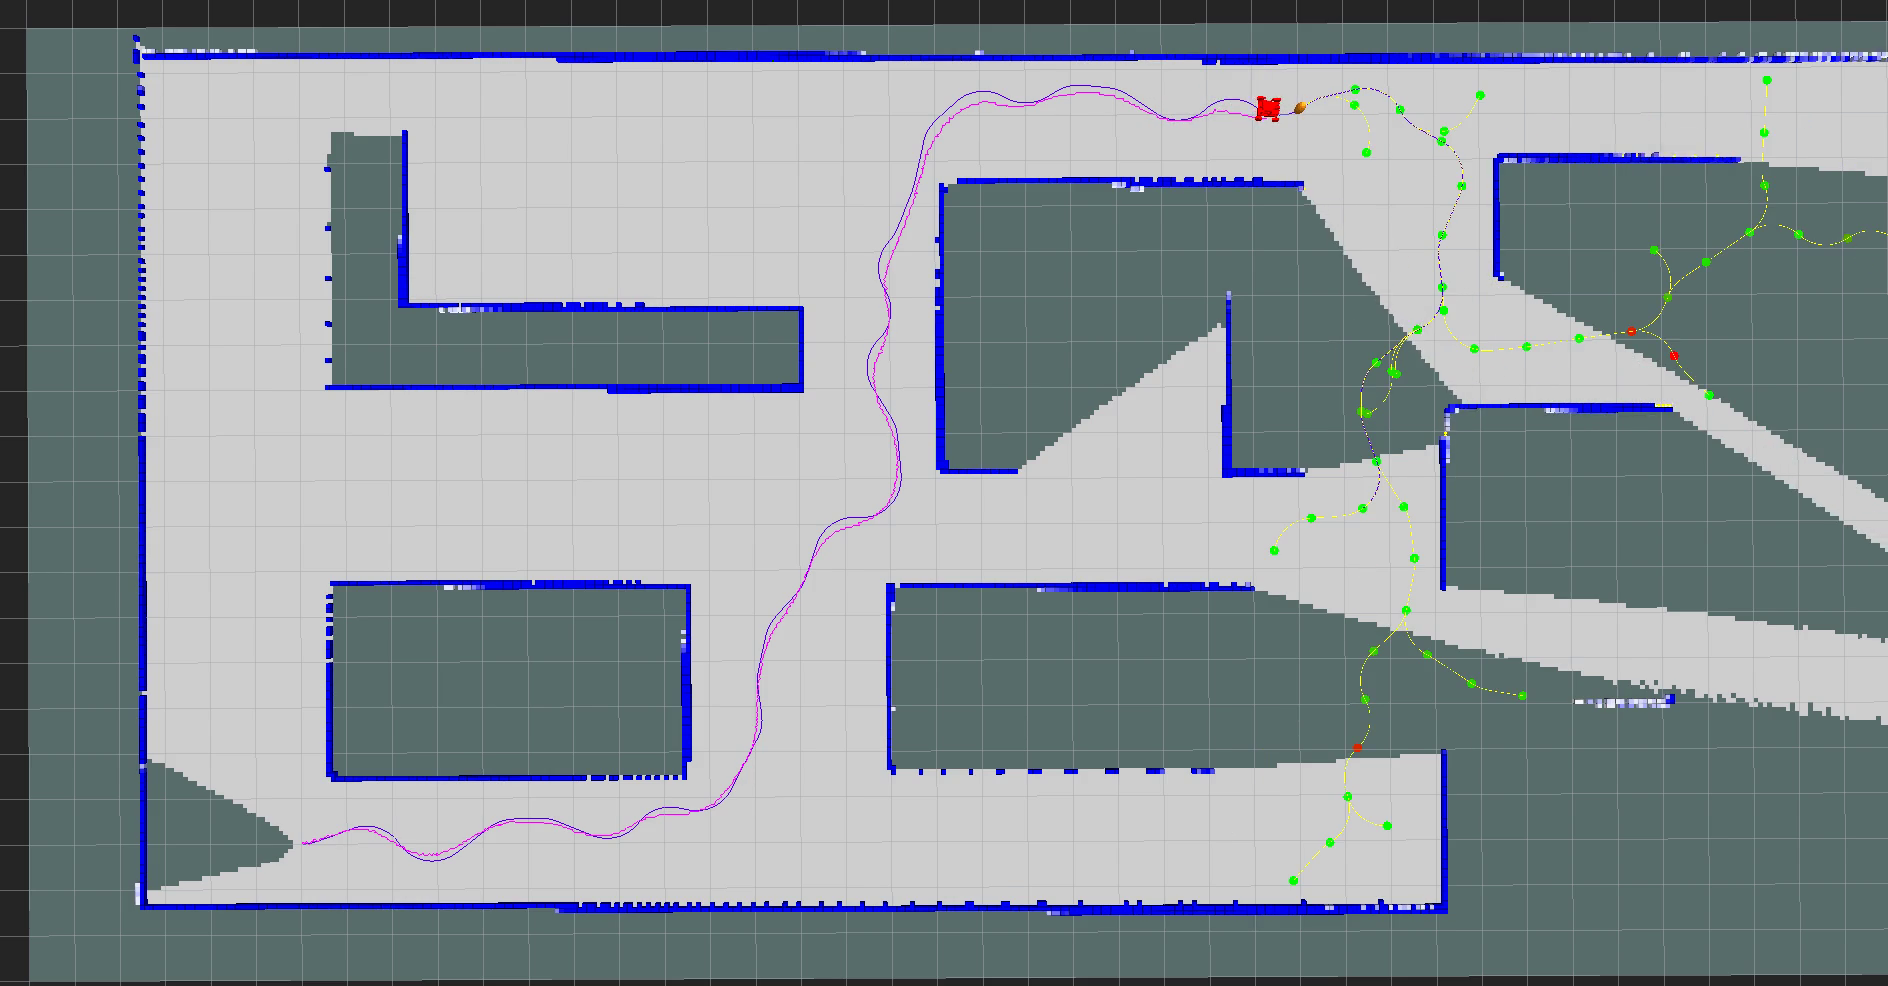
\includegraphics[width=0.9\textwidth]{largemap_frame3.png}
	\caption{Planner expands into new regions as the map expands \label{fig:largemap_frame3}}
	\end{subfigure}
	\begin{subfigure}{0.49\textwidth}
	\centering
	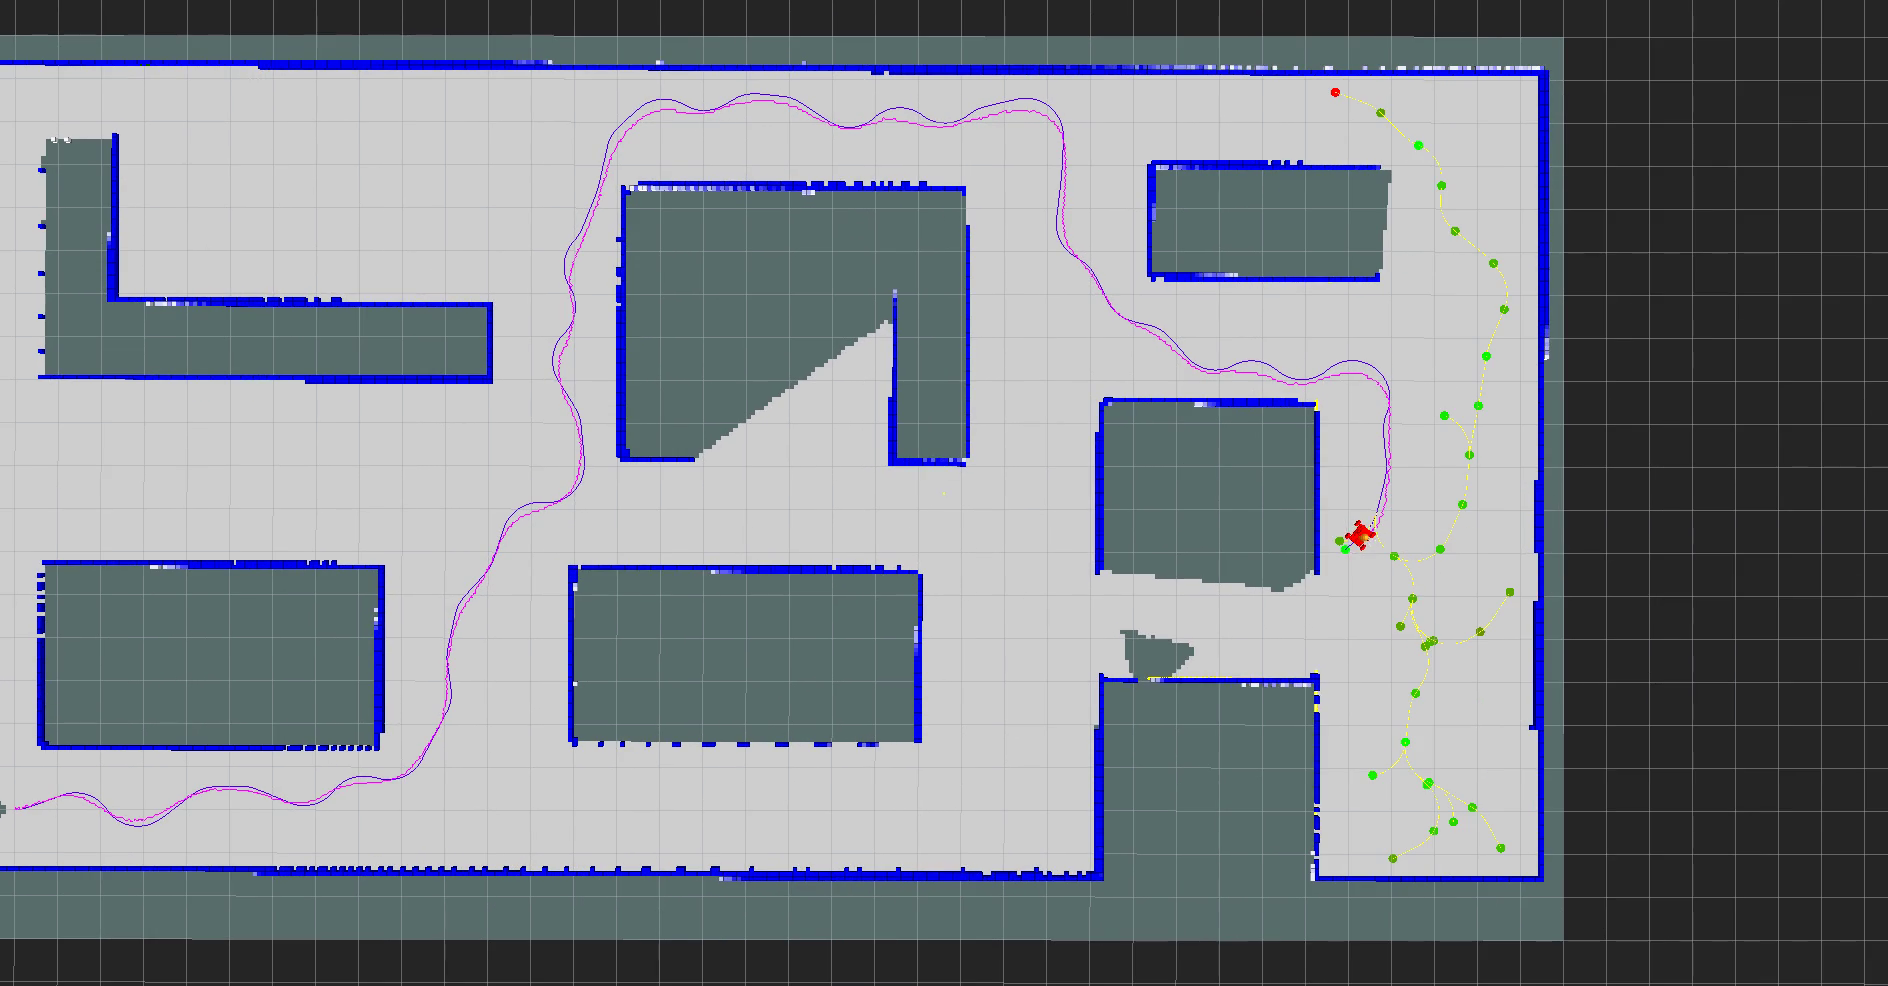
\includegraphics[width=0.9\textwidth]{largemap_frame4.png}
	\caption{Robot has autonomously mapped most of the environment \label{fig:largemap_frame4}}
	\end{subfigure}
	
	\vspace*{0.2in}

	\begin{subfigure}{0.6\textwidth}
	\centering
	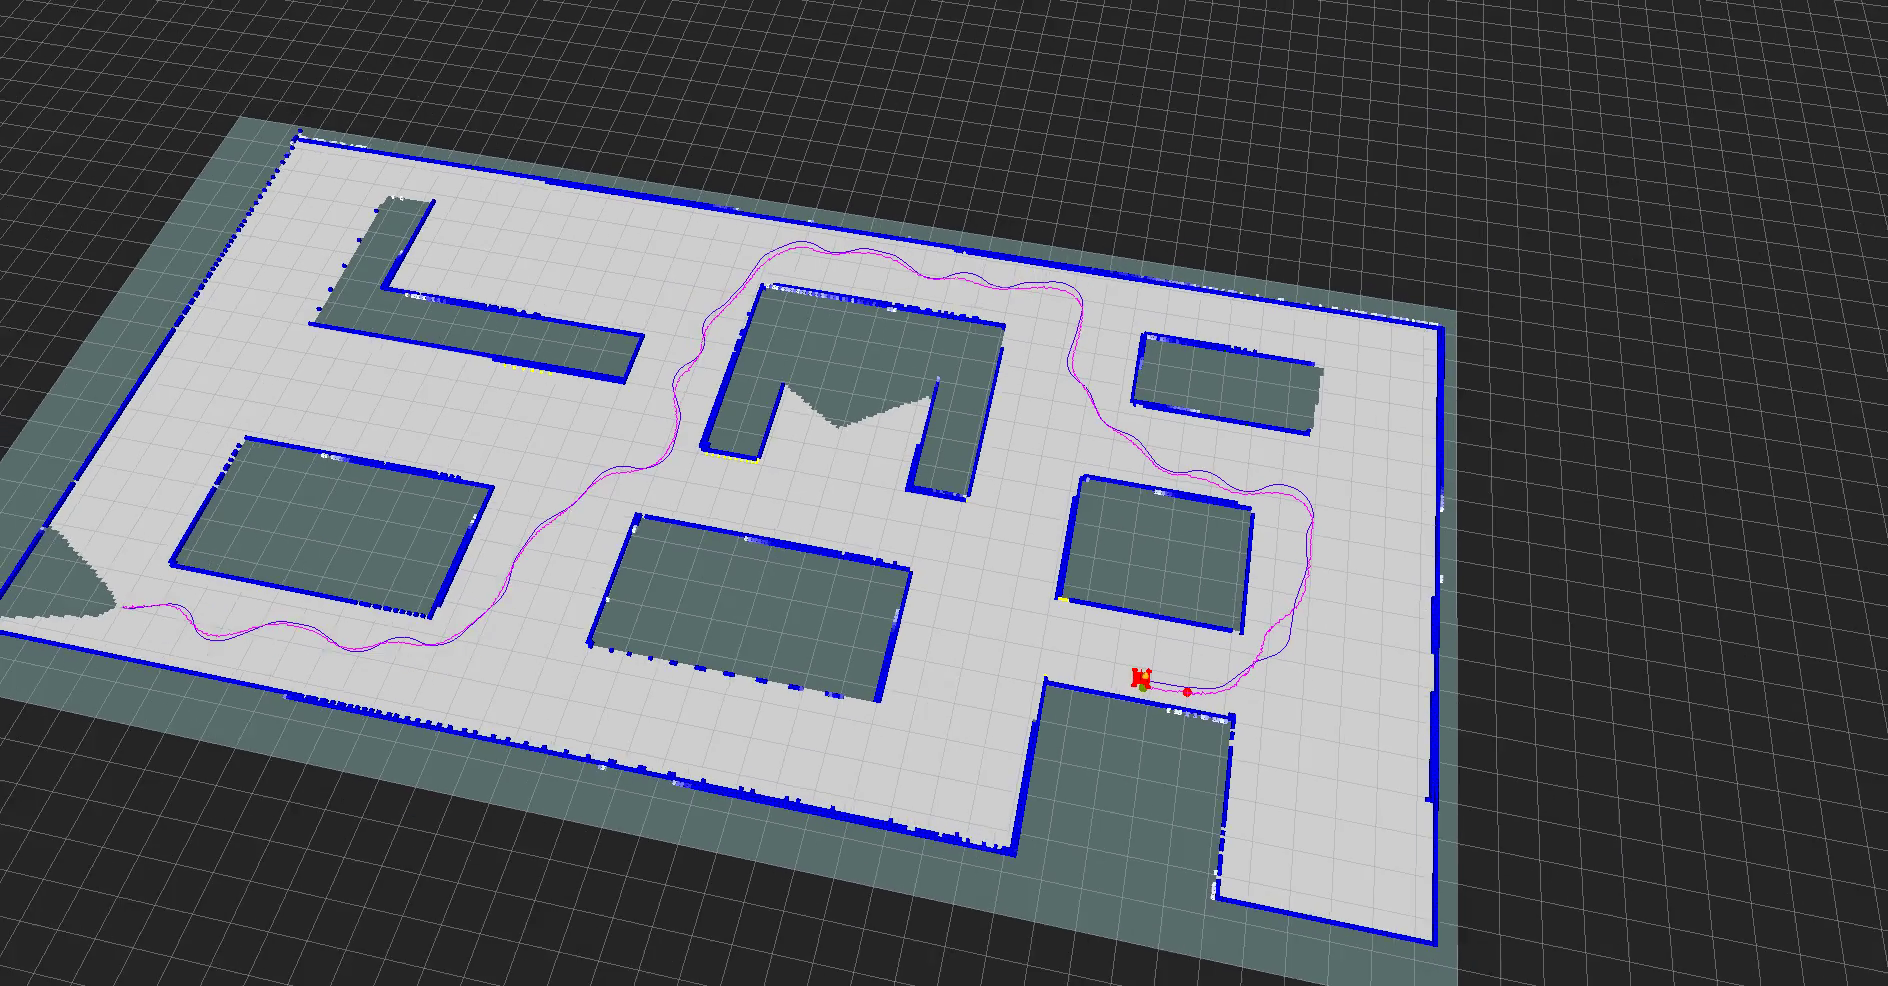
\includegraphics[width=0.9\textwidth]{largemap_frame5.png}
	\caption{Final map \label{fig:largemap_frame5}}
	\end{subfigure}
	
	\caption{Snapshots of the ground robot exploring a large unknown environment. \label{fig:largemap_snapshots}}
\end{figure*}